\paragraph{CSE572 Statistical Machine Learning - Project 3 - Classification Using Neural Networks and Deep Learning Project}

\subparagraph{Import Libraries}

\begin{verbatim}
import warnings
warnings.filterwarnings("ignore")
import keras
from tensorflow.keras.utils import to_categorical
from keras.datasets import mnist
from keras.models import Sequential
from keras.layers import Dense, Dropout, Flatten
from keras.layers import Conv2D, MaxPooling2D
from keras import backend as K
import tensorflow as tf

from sklearn.metrics import classification_report
from sklearn.metrics import confusion_matrix, ConfusionMatrixDisplay

import os
import multiprocessing

import numpy as np
import pandas as pd
import matplotlib.pyplot as plt
\end{verbatim}

\subparagraph{Problem Solution}

\subparagraph{Show Compute Environment}

\begin{verbatim}
# Number of logical CPUs
num_cores = multiprocessing.cpu_count()
print(f"Number of CPU cores available: {num_cores}")

# Number of GPUs
print("Num GPUs Available:", len(tf.config.list_physical_devices('GPU')))
\end{verbatim}

\begin{verbatim}
Number of CPU cores available: 16
Num GPUs Available: 1
\end{verbatim}

\subparagraph{Define Batch Size}

\begin{verbatim}
batch_size = 64
\end{verbatim}

\subparagraph{Define Number of Classes}

\begin{verbatim}
num_classes = 10
\end{verbatim}

\subparagraph{Define Number of Training Epochs}

\begin{verbatim}
epochs = 12
\end{verbatim}

\subparagraph{Define Image Dimensions}

\begin{verbatim}
# input image dimensions
img_rows, img_cols = 28, 28
\end{verbatim}

\subparagraph{Define Kernel Size (Updated from (3,3) Baseline to (5,5) Task 2)}

\begin{verbatim}
kernel_size = (5,5)
\end{verbatim}

\subparagraph{Define Pooling Size}

\begin{verbatim}
pool_size = (2,2)
\end{verbatim}

\subparagraph{Load Data and Train / Test Split}

\begin{verbatim}
# the data, split between train and test sets
(x_train, y_train), (x_test, y_test)=tf.keras.datasets.mnist.load_data('mnist.npz')
\end{verbatim}

\begin{verbatim}
x_train.shape
\end{verbatim}

\begin{verbatim}
(60000, 28, 28)
\end{verbatim}

\begin{verbatim}
y_train.shape
\end{verbatim}

\begin{verbatim}
(60000,)
\end{verbatim}

\begin{verbatim}
x_test.shape
\end{verbatim}

\begin{verbatim}
(10000, 28, 28)
\end{verbatim}

\begin{verbatim}
y_test.shape
\end{verbatim}

\begin{verbatim}
(10000,)
\end{verbatim}

\subparagraph{EDA on Data}

\subparagraph{Visualize First Train Image}

\begin{verbatim}
ticks = np.arange(0, 28+2, 2)
#ticks
\end{verbatim}

\begin{verbatim}
plt.imshow(x_train[0], cmap='grey')
plt.xlim(0, 28)
plt.xticks(ticks=ticks)
plt.yticks(ticks=ticks)
plt.show()
\end{verbatim}

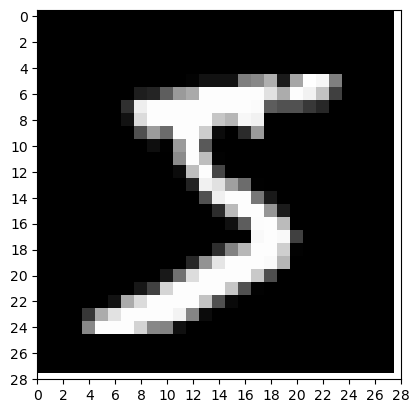
\includegraphics[width=0.7\linewidth]{files/6307c9063d2a896beafa2689ed8da5df.png}

\subparagraph{Visualize the First 10 X Train Images}

\begin{verbatim}
# Display the first 10 images
num_images_to_display = 10
plt.figure(figsize=(10, 5))  # Adjust the figure size

for i in range(num_images_to_display):
    plt.subplot(2, 5, i + 1)  # Create a 2x5 grid for 10 images
    plt.imshow(x_train[i], cmap='gray')  # Display each image
    plt.title(f'Train Image {i + 1}')
    plt.axis('off')  # Hide axes for better visualization

plt.tight_layout()
plt.show()
\end{verbatim}

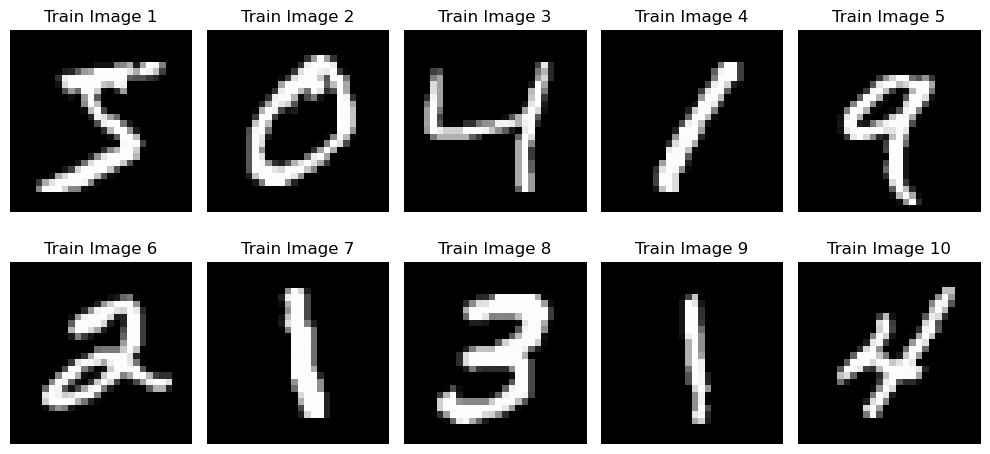
\includegraphics[width=0.7\linewidth]{files/7ce587a1409319f6f079817b9548c2b6.png}

\subparagraph{Print the First 10 Y Train Class Labels}

\begin{verbatim}
y_train[0:10]
\end{verbatim}

\begin{verbatim}
array([5, 0, 4, 1, 9, 2, 1, 3, 1, 4], dtype=uint8)
\end{verbatim}

\subparagraph{Visualize the First X 10 Test Images}

\begin{verbatim}
# Display the first 10 images
num_images_to_display = 10
plt.figure(figsize=(10, 5))  # Adjust the figure size

for i in range(num_images_to_display):
    plt.subplot(2, 5, i + 1)  # Create a 2x5 grid for 10 images
    plt.imshow(x_test[i], cmap='gray')  # Display each image
    plt.title(f'Test Image {i + 1}')
    plt.axis('off')  # Hide axes for better visualization

plt.tight_layout()
plt.show()
\end{verbatim}

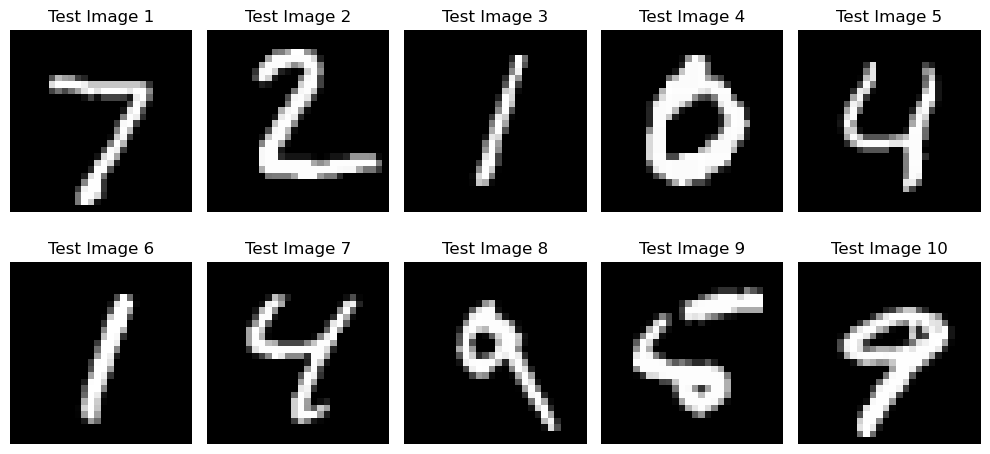
\includegraphics[width=0.7\linewidth]{files/0e370b8936aebd53b2df30837226df74.png}

\subparagraph{Print the First 10 Y Test Class Labels}

\begin{verbatim}
y_test[0:10]
\end{verbatim}

\begin{verbatim}
array([7, 2, 1, 0, 4, 1, 4, 9, 5, 9], dtype=uint8)
\end{verbatim}

\subparagraph{Reformat Data if Necessary}

\begin{verbatim}
if K.image_data_format() == 'channels_first':
    x_train = x_train.reshape(x_train.shape[0], 1, img_rows, img_cols)
    x_test = x_test.reshape(x_test.shape[0], 1, img_rows, img_cols)
    input_shape = (1, img_rows, img_cols)
else:
    x_train = x_train.reshape(x_train.shape[0], img_rows, img_cols, 1)
    x_test = x_test.reshape(x_test.shape[0], img_rows, img_cols, 1)
    input_shape = (img_rows, img_cols, 1)
\end{verbatim}

\begin{verbatim}
x_train.shape
\end{verbatim}

\begin{verbatim}
(60000, 28, 28, 1)
\end{verbatim}

\begin{verbatim}
x_test.shape
\end{verbatim}

\begin{verbatim}
(10000, 28, 28, 1)
\end{verbatim}

\subparagraph{Cast and Normalize Data}

\begin{verbatim}
x_train = x_train.astype('float32')
x_test = x_test.astype('float32')
x_train /= 255
x_test /= 255
\end{verbatim}

\subparagraph{Print Out Description of Data}

\begin{verbatim}
print('x_train shape:', x_train.shape)
print(x_train.shape[0], 'train samples')
print(x_test.shape[0], 'test samples')
\end{verbatim}

\begin{verbatim}
x_train shape: (60000, 28, 28, 1)
60000 train samples
10000 test samples
\end{verbatim}

\subparagraph{Convert Class Vectors into Binary Class Matrices}

\begin{verbatim}
# convert class vectors to binary class matrices
y_train = to_categorical(y_train, num_classes)
y_test = to_categorical(y_test, num_classes)
\end{verbatim}

\begin{verbatim}
y_train.shape
\end{verbatim}

\begin{verbatim}
(60000, 10)
\end{verbatim}

\begin{verbatim}
y_train[0:5]
\end{verbatim}

\begin{verbatim}
array([[0., 0., 0., 0., 0., 1., 0., 0., 0., 0.],
       [1., 0., 0., 0., 0., 0., 0., 0., 0., 0.],
       [0., 0., 0., 0., 1., 0., 0., 0., 0., 0.],
       [0., 1., 0., 0., 0., 0., 0., 0., 0., 0.],
       [0., 0., 0., 0., 0., 0., 0., 0., 0., 1.]], dtype=float32)
\end{verbatim}

\begin{verbatim}
y_test.shape
\end{verbatim}

\begin{verbatim}
(10000, 10)
\end{verbatim}

\begin{verbatim}
y_test[0:5]
\end{verbatim}

\begin{verbatim}
array([[0., 0., 0., 0., 0., 0., 0., 1., 0., 0.],
       [0., 0., 1., 0., 0., 0., 0., 0., 0., 0.],
       [0., 1., 0., 0., 0., 0., 0., 0., 0., 0.],
       [1., 0., 0., 0., 0., 0., 0., 0., 0., 0.],
       [0., 0., 0., 0., 1., 0., 0., 0., 0., 0.]], dtype=float32)
\end{verbatim}

\subparagraph{Create Task 2 Model}

\subparagraph{Define Task 2 Model Type}

\begin{verbatim}
# Artificial Neural Network
model = Sequential()
\end{verbatim}

\begin{verbatim}
model
\end{verbatim}

\begin{verbatim}
<keras.engine.sequential.Sequential at 0x24a43f95730>
\end{verbatim}

\subparagraph{Create Task 2 Model Structure}

\begin{verbatim}
# First layer is a convolutional layer with 6 filters, each of size 3x3
model.add(Conv2D(
    filters=6, 
    kernel_size=kernel_size,
    strides=(1, 1),
    activation='relu',
    input_shape=input_shape))

# Second layer is a max pooling layer with a pool size of 2x2
model.add(MaxPooling2D(
    pool_size=pool_size,
    strides=(1, 1)))

# Third layer is a convolutional layer with 16 filters, each of size 3x3
model.add(Conv2D(
    filters=16, 
    kernel_size=kernel_size,
    strides=(1, 1),
    activation='relu'))

# Fourth layer is a max pooling layer with a pool size of 2x2
model.add(MaxPooling2D(
    pool_size=pool_size,
    strides=(1, 1)))

# Fifth layer is a flatten layer
model.add(Flatten())

# Sixth layer is a dense layer with 120 units
model.add(Dense(120, activation='relu'))

# Seventh layer is a dense layer with 84 units
model.add(Dense(84, activation='relu'))

# Eighth layer is a dense layer with 10 units for 10 classes in the output layer
model.add(Dense(num_classes, activation='softmax'))
\end{verbatim}

\begin{verbatim}
model
\end{verbatim}

\begin{verbatim}
<keras.engine.sequential.Sequential at 0x24a43f95730>
\end{verbatim}

\subparagraph{Define Task 2 Model Optimizer}

\begin{verbatim}
optim = tf.keras.optimizers.Adadelta(
    learning_rate=0.1, 
    rho=0.95, 
    decay=0.0)
\end{verbatim}

\begin{verbatim}
optim
\end{verbatim}

\begin{verbatim}
<keras.optimizer_v2.adadelta.Adadelta at 0x24a42d01fd0>
\end{verbatim}

\subparagraph{Compile Task 2 Model}

\begin{verbatim}
# https://keras.io/optimizers/ 
model.compile(loss=keras.losses.categorical_crossentropy,
              optimizer=optim,
              metrics=['accuracy'])
\end{verbatim}

\begin{verbatim}
model
\end{verbatim}

\begin{verbatim}
<keras.engine.sequential.Sequential at 0x24a43f95730>
\end{verbatim}

\subparagraph{Train Task 2 Model}

\begin{verbatim}
model_history = \
    model.fit(x_train, y_train,
          batch_size=batch_size,
          epochs=epochs,
          verbose=2,
          validation_data=(x_test, y_test))
\end{verbatim}

\begin{verbatim}
Epoch 1/12
938/938 - 10s - loss: 0.3448 - accuracy: 0.8967 - val_loss: 0.1091 - val_accuracy: 0.9694
Epoch 2/12
938/938 - 2s - loss: 0.0940 - accuracy: 0.9723 - val_loss: 0.0704 - val_accuracy: 0.9806
Epoch 3/12
938/938 - 2s - loss: 0.0659 - accuracy: 0.9804 - val_loss: 0.0575 - val_accuracy: 0.9809
Epoch 4/12
938/938 - 2s - loss: 0.0530 - accuracy: 0.9841 - val_loss: 0.0489 - val_accuracy: 0.9841
Epoch 5/12
938/938 - 2s - loss: 0.0451 - accuracy: 0.9865 - val_loss: 0.0571 - val_accuracy: 0.9808
Epoch 6/12
938/938 - 2s - loss: 0.0392 - accuracy: 0.9887 - val_loss: 0.0464 - val_accuracy: 0.9847
Epoch 7/12
938/938 - 2s - loss: 0.0352 - accuracy: 0.9895 - val_loss: 0.0358 - val_accuracy: 0.9885
Epoch 8/12
938/938 - 2s - loss: 0.0318 - accuracy: 0.9908 - val_loss: 0.0366 - val_accuracy: 0.9875
Epoch 9/12
938/938 - 2s - loss: 0.0291 - accuracy: 0.9911 - val_loss: 0.0323 - val_accuracy: 0.9889
Epoch 10/12
938/938 - 2s - loss: 0.0265 - accuracy: 0.9923 - val_loss: 0.0316 - val_accuracy: 0.9892
Epoch 11/12
938/938 - 2s - loss: 0.0240 - accuracy: 0.9930 - val_loss: 0.0335 - val_accuracy: 0.9887
Epoch 12/12
938/938 - 2s - loss: 0.0222 - accuracy: 0.9937 - val_loss: 0.0344 - val_accuracy: 0.9894
\end{verbatim}

\begin{verbatim}
model_history.history['loss']
\end{verbatim}

\begin{verbatim}
[0.34479445219039917,
 0.09400391578674316,
 0.0658968836069107,
 0.05295504257082939,
 0.04514137655496597,
 0.03916701301932335,
 0.03520461171865463,
 0.03181973844766617,
 0.029129598289728165,
 0.026451660320162773,
 0.024046970531344414,
 0.022170674055814743]
\end{verbatim}

\begin{verbatim}
model_history.history['accuracy']
\end{verbatim}

\begin{verbatim}
[0.8967000246047974,
 0.9722999930381775,
 0.9804333448410034,
 0.9841333627700806,
 0.9865333437919617,
 0.9887333512306213,
 0.9895333051681519,
 0.9907500147819519,
 0.9910500049591064,
 0.9922666549682617,
 0.992983341217041,
 0.9937000274658203]
\end{verbatim}

\subparagraph{Save the Fitted Task 2 Model}

\begin{verbatim}
model.save("fitted_task2_model.keras")  # Save the model in HDF5 format

# Save the history
import json
with open("fitted_task2_model_history.json", "w") as f:
    json.dump(model_history.history, f)
\end{verbatim}

\subparagraph{Load the Model if Necessary}

\begin{verbatim}
#from keras.models import load_model

#model = load_model("fitted_baseline_model.keras")  # Load the saved model

# Load the history
#import json
#with open("fitted_baseline_model_history.json", "r") as f:
#    model_history = json.load(f)
\end{verbatim}

\subparagraph{Get Model Summary}

\begin{verbatim}
model.summary()
\end{verbatim}

\begin{verbatim}
Model: "sequential"
_________________________________________________________________
Layer (type)                 Output Shape              Param #   
=================================================================
conv2d (Conv2D)              (None, 24, 24, 6)         156       
_________________________________________________________________
max_pooling2d (MaxPooling2D) (None, 23, 23, 6)         0         
_________________________________________________________________
conv2d_1 (Conv2D)            (None, 19, 19, 16)        2416      
_________________________________________________________________
max_pooling2d_1 (MaxPooling2 (None, 18, 18, 16)        0         
_________________________________________________________________
flatten (Flatten)            (None, 5184)              0         
_________________________________________________________________
dense (Dense)                (None, 120)               622200    
_________________________________________________________________
dense_1 (Dense)              (None, 84)                10164     
_________________________________________________________________
dense_2 (Dense)              (None, 10)                850       
=================================================================
Total params: 635,786
Trainable params: 635,786
Non -trainable params: 0
_________________________________________________________________
\end{verbatim}

\subparagraph{Evaluate Task 2 Model}

\subparagraph{Training Accuracy}

\begin{verbatim}
loss_train, accuracy_train = model.evaluate(x_train, y_train)
\end{verbatim}

\begin{verbatim}
1875/1875 [==============================] - 3s 1ms/step - loss: 0.0209 - accuracy: 0.9940
\end{verbatim}

\begin{verbatim}
print('Print the training loss and the accuracy of the model on the dataset')
print('Train Loss: {0:0.4f} Train Accuracy: {1:0.4f}'.format(loss_train, accuracy_train))
\end{verbatim}

\begin{verbatim}
Print the training loss and the accuracy of the model on the dataset
Train Loss: 0.0209 Train Accuracy: 0.9940
\end{verbatim}

\subparagraph{Testing Accuracy}

\begin{verbatim}
loss_test, accuracy_test = model.evaluate(x_test, y_test)
\end{verbatim}

\begin{verbatim}
313/313 [==============================] - 1s 2ms/step - loss: 0.0344 - accuracy: 0.9894
\end{verbatim}

\begin{verbatim}
print('Print the testing loss and the accuracy of the model on the dataset')
print('Test Loss: {0:0.4f} Test Accuracy: {1:0.4f}'.format(loss_test, accuracy_test))
\end{verbatim}

\begin{verbatim}
Print the testing loss and the accuracy of the model on the dataset
Test Loss: 0.0344 Test Accuracy: 0.9894
\end{verbatim}

\begin{verbatim}
#score = model.evaluate(x_test, y_test, verbose=0)
#print('Test loss:', score[0])
#print('Test accuracy:', score[1])
\end{verbatim}

\subparagraph{Use Model to Make Predictions}

\begin{verbatim}
########################################
# Making predictions and evaluating the model
#######################################

# Predicting the Test set results
y_pred = model.predict(x_test)
y_pred[y_pred > 0.9] = 1
\end{verbatim}

\begin{verbatim}
y_pred[y_pred > 0.9] = 1
y_pred[y_pred <= 0.9] = 0
\end{verbatim}

\begin{verbatim}
y_pred.shape
\end{verbatim}

\begin{verbatim}
(10000, 10)
\end{verbatim}

\begin{verbatim}
y_pred[0]
\end{verbatim}

\begin{verbatim}
array([0., 0., 0., 0., 0., 0., 0., 1., 0., 0.], dtype=float32)
\end{verbatim}

\begin{verbatim}
# summarize the middle 5 cases in a table

for i in range(15,20):
    print('actual   ', end=' ')
    for j in range(10):
        print('{:.1f}'.format(y_test[i][j]), end=' ')
    print()
    print('predicted', end=' ')
    for j in range(10):
        print('{:.1f}'.format(y_pred[i][j]), end=' ')
    print()
    print()
\end{verbatim}

\begin{verbatim}
actual    0.0 0.0 0.0 0.0 0.0 1.0 0.0 0.0 0.0 0.0 
predicted 0.0 0.0 0.0 0.0 0.0 1.0 0.0 0.0 0.0 0.0 

actual    0.0 0.0 0.0 0.0 0.0 0.0 0.0 0.0 0.0 1.0 
predicted 0.0 0.0 0.0 0.0 0.0 0.0 0.0 0.0 0.0 1.0 

actual    0.0 0.0 0.0 0.0 0.0 0.0 0.0 1.0 0.0 0.0 
predicted 0.0 0.0 0.0 0.0 0.0 0.0 0.0 1.0 0.0 0.0 

actual    0.0 0.0 0.0 1.0 0.0 0.0 0.0 0.0 0.0 0.0 
predicted 0.0 0.0 0.0 1.0 0.0 0.0 0.0 0.0 0.0 0.0 

actual    0.0 0.0 0.0 0.0 1.0 0.0 0.0 0.0 0.0 0.0 
predicted 0.0 0.0 0.0 0.0 1.0 0.0 0.0 0.0 0.0 0.0
\end{verbatim}

\subparagraph{Making the Confusion Matrix}

\begin{verbatim}
y_pred[0]
\end{verbatim}

\begin{verbatim}
array([0., 0., 0., 0., 0., 0., 0., 1., 0., 0.], dtype=float32)
\end{verbatim}

\begin{verbatim}
y_test[0]
\end{verbatim}

\begin{verbatim}
array([0., 0., 0., 0., 0., 0., 0., 1., 0., 0.], dtype=float32)
\end{verbatim}

\begin{verbatim}
y_pred.shape
\end{verbatim}

\begin{verbatim}
(10000, 10)
\end{verbatim}

\begin{verbatim}
y_test.shape
\end{verbatim}

\begin{verbatim}
(10000, 10)
\end{verbatim}

\begin{verbatim}
# Convert one -hot encoded arrays to label indices
y_pred_labels = np.argmax(y_pred, axis=1)
y_test_labels = np.argmax(y_test, axis=1)
\end{verbatim}

\begin{verbatim}
y_pred_labels[0:15]
\end{verbatim}

\begin{verbatim}
array([7, 2, 1, 0, 4, 1, 4, 9, 5, 9, 0, 6, 9, 0, 1], dtype=int64)
\end{verbatim}

\begin{verbatim}
y_test_labels[0:15]
\end{verbatim}

\begin{verbatim}
array([7, 2, 1, 0, 4, 1, 4, 9, 5, 9, 0, 6, 9, 0, 1], dtype=int64)
\end{verbatim}

\begin{verbatim}
# Making the Confusion Matrix
cm = confusion_matrix(y_test_labels, y_pred_labels)
print('Print the Confusion Matrix:')
print(cm)
\end{verbatim}

\begin{verbatim}
Print the Confusion Matrix:
[[ 977    0    0    0    0    0    1    1    1    0]
 [   8 1127    0    0    0    0    0    0    0    0]
 [  30    2  998    0    1    0    0    1    0    0]
 [  25    0    0  985    0    0    0    0    0    0]
 [  30    0    0    0  951    0    0    0    0    1]
 [  23    0    0    1    0  867    1    0    0    0]
 [  34    1    0    0    1    3  919    0    0    0]
 [  31    0    1    0    0    0    0  996    0    0]
 [  56    0    2    1    0    0    0    2  911    2]
 [  41    2    0    0    1    0    0    0    0  965]]
\end{verbatim}

\begin{verbatim}
print(classification_report(y_test_labels, y_pred_labels))
\end{verbatim}

\begin{verbatim}
precision    recall  f1 -score   support

           0       0.78      1.00      0.87       980
           1       1.00      0.99      0.99      1135
           2       1.00      0.97      0.98      1032
           3       1.00      0.98      0.99      1010
           4       1.00      0.97      0.98       982
           5       1.00      0.97      0.98       892
           6       1.00      0.96      0.98       958
           7       1.00      0.97      0.98      1028
           8       1.00      0.94      0.97       974
           9       1.00      0.96      0.98      1009

    accuracy                           0.97     10000
   macro avg       0.98      0.97      0.97     10000
weighted avg       0.98      0.97      0.97     10000
\end{verbatim}

\begin{verbatim}
disp = ConfusionMatrixDisplay(confusion_matrix=cm, display_labels=np.arange(10))
disp.plot()
plt.savefig('confusion_matrix_baseline.png')
plt.show()
\end{verbatim}

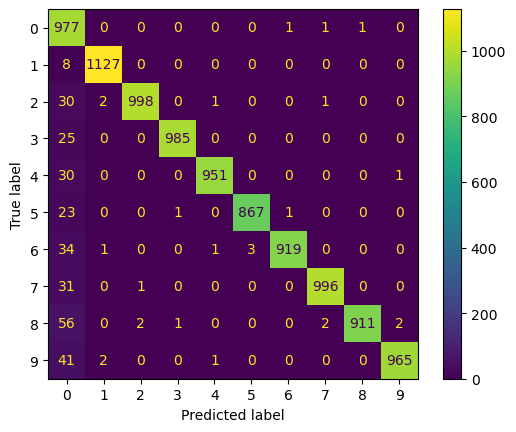
\includegraphics[width=0.7\linewidth]{files/fd43804ac8b6851f52b02e2fd04b6cf6.png}

\subparagraph{Plot The Accuracy}

\begin{verbatim}
print('Plot the accuracy')
# Keras 2.2.4 recognizes 'acc' and 2.3.1 recognizes 'accuracy'
# use the command python -c 'import keras; print(keras.__version__)' on MAC or Linux to check Keras' version
plt.plot(model_history.history['accuracy'], label='Training Accuracy')
#plt.plot(model_history.history['val_accuracy'], label='Validation Accuracy')
plt.title('5x5 Kernel Model Accuracy')
plt.ylabel('Accuracy')
plt.xlabel('Epoch')
plt.yticks(np.arange(0.9, 1.2, step=0.01))
plt.xticks(np.arange(0, 14, step=1))
plt.ylim(0.9, 1)
plt.xlim(0, 12)
plt.grid()
plt.legend(loc='lower right')
plt.savefig('task2_model_accuracy.png')
plt.show()
\end{verbatim}

\begin{verbatim}
Plot the accuracy
\end{verbatim}

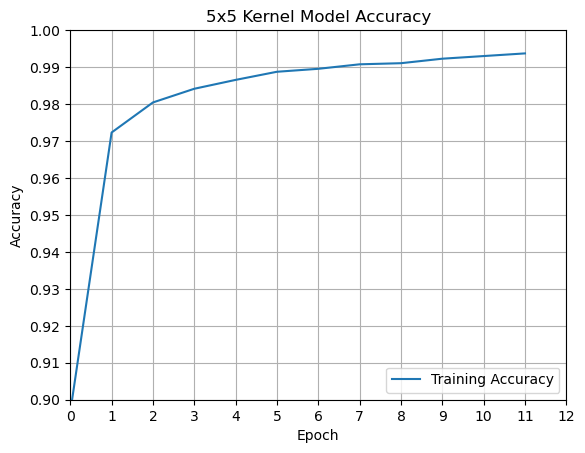
\includegraphics[width=0.7\linewidth]{files/6bf65c0e421032d74a4445f892d110fe.png}

\subparagraph{Plot the Loss}

\begin{verbatim}
print('Plot the loss')
plt.plot(model_history.history['loss'], label='Training Loss')
#plt.plot(model_history.history['val_loss'], label='Validation Loss')
plt.title('5x5 Kernel Model Loss')
plt.ylabel('Loss')
plt.xlabel('Epoch')
plt.yticks(np.arange(0, 0.40, step=0.025))
plt.xticks(np.arange(0, 14, step=1))
plt.ylim(0, 0.35)
plt.xlim(0, 12)
plt.grid()
plt.legend(loc='upper right')
plt.savefig('task2_model_loss.png')
plt.show()
\end{verbatim}

\begin{verbatim}
Plot the loss
\end{verbatim}

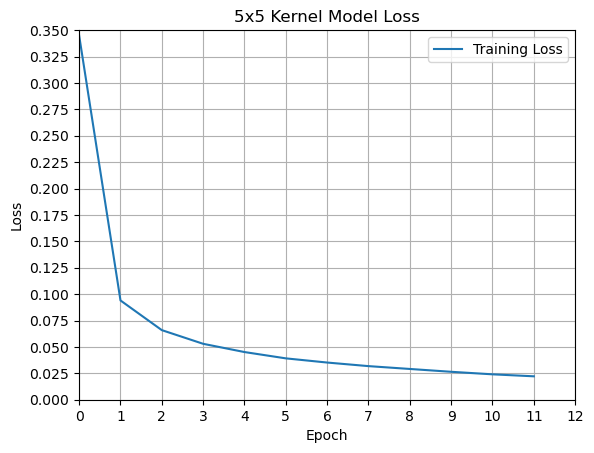
\includegraphics[width=0.7\linewidth]{files/c291a9c8546889c28e64337088e46501.png}